%%&proposal
\documentclass[simple]{mybeamer}

\title{Plagiarism checker}
\subtitle{Textindexierung}
\date{7th of July 2013}
\author{Daniel Hoske \and Stefan Walzer \and Geoffroy Deneuville}

\usetikzlibrary{arrows}
\tikzset{
    boxed/.style={draw, rectangle, minimum width=3cm, minimum height=0.6cm, thick,
                  text height=1.5ex,text depth=0.5ex},
    boxed marked/.style={boxed, fill=red, text=white},
    every edge/.style={draw, thick, -latex, shorten >=3, shorten <=3}
}
\lstset{basicstyle=\ttfamily\tiny,numbers=none}

% bibliography
\usepackage[backref,style=numeric,url=false,backend=biber,hyperref=true]{biblatex}
\addbibresource{../bibliography.bib}
\nocite{*}

\begin{document}
\maketitle

\begin{frame}{Goal}
    Goal:
    \begin{itemize}
      \item Software for analysing whether a document is a plagiarism
      \item Visualization of results for manual testing
      \item Answer $1$-to-$n$ queries: Given a large set of reference documents~$D$ and a query document~$q$, does $q$ plagiarise one of the documents in~$D$?
    \end{itemize}

    \pause

    Approach:
    \begin{itemize}
      \item Compute similarity score of~$q$ with every document~$d \in D$ s.th. higher
      scores signify a higher chance of plagiarism
      \item[$\Rightarrow$] Can only preselect likely plagiarisms for manual checking
    \end{itemize}
\end{frame}

\begin{frame}{Contents}
  \tableofcontents
\end{frame}

\section{Algorithms}

\begin{frame}{Overview}

    \begin{center}
        \begin{tikzpicture}
          \tikzset{b1/.style={boxed},b2/.style={boxed},b3/.style={boxed},b4/.style={boxed}}
          \only<1>{\tikzset{b1/.style={boxed marked}}}
          \only<2>{\tikzset{b2/.style={boxed marked}}}
          \only<3>{\tikzset{b3/.style={boxed marked}}}
          \only<4>{\tikzset{b4/.style={boxed marked}}}
        
          \draw (0, 0)  node[b1] (norm)    {Normalisation}
                (4, -1) node[b3] (ranking) {Ranking}
                (4, 1)  node[b2] (fp)      {Fingerprinting}
                (8, 0)  node[b4] (vis)     {Visualization};
          \draw (norm) edge (fp.west) 
                (norm) edge (ranking.west)
                (fp.east)   edge (vis)
                (ranking.east) edge (vis);
        \end{tikzpicture}
    \end{center}

    \begin{overprint}
      \onslide<1>\vspace{0.5cm}
        Parse text into words and remove stop words
      \onslide<2>\vspace{0.5cm}
        Compact description (fingerprint) of query that can be compared
        to the fingerprints of the references
      \onslide<3>\vspace{0.5cm}
        Similarity measures based on word frequencies in the texts
      \onslide<4>\vspace{0.5cm}
        Visual report for manually checking the relevance of the results
    \end{overprint}
    \vspace{0.25cm}
    \hrule
    \vspace{0.25cm}Based on Hoad and Zobel, 2003.
\end{frame}

%\begin{frame}{Normalisation}
%\begin{itemize}
%    \item Input: unstructured ASCII text~$q$
%    \item<2-> Parse into words
%    \item<2-> Transform to lower case
%    \item<2-> Remove stop words
%    \item Output: normalised text~$\widetilde{q}$, index from $\widetilde{q}$ to~$q$
%\end{itemize}
%\end{frame}

\begin{frame}{Ranking}
  Variants of frequency based measures between $q$ and~$d$:
  \begin{center}
      {\lnfigures\setlength{\extrarowheight}{0.5\baselineskip}
      \begin{tabular}{l|r@{$\cdot$}lp{0.5\linewidth}}
      1 & $\frac{\text{1}}{\text{1}+|f_d-f_q|}$ & $\sum_{t\in{q\cap d}} \frac{\ln(N/f_t)}{\text{1}+|f_{d,t}-f_{q,t}|} $\\
      2 & $\frac{\text{1}}{\text{1}+\ln(\text{1} + |f_d-f_q|)}$ & $\sum_{t\in{q\cap d}} \frac{\ln(\text{1} + N/f_t)}{\text{1}+|f_{d,t}-f_{q,t}|} $\\
      3 & $\frac{\text{1}}{\text{1}+\ln(\text{1} + |f_d-f_q|)}$ & $\sum_{t\in{q\cap d}} \frac{\ln(\text{1} + N/f_t)\cdot(f_{d,t}+f_{q,t})}{\text{1}+|f_{d,t}-f_{q,t}|} $\\
      4 & $\frac{\text{1}}{\text{1}+\ln(\text{1} + |f_d-f_q|)}$ & $\sum_{t\in{q\cap d}} \frac{\ln(N/f_t)}{\text{1}+|f_{d,t}-f_{q,t}|} $\\
      5 & $\frac{\text{1}}{\text{1}+\ln(\text{1} + |f_d-f_q|)}$ & $\sum_{t\in{q\cap d}} \frac{N/f_t}{\text{1}+|f_{d,t}-f_{q,t}|} $\\
      \end{tabular}}
  \end{center}
  \vfill
  Glossary:\\
  \scalebox{0.6}{
  \begin{minipage}{\linewidth}
      \begin{tabular}{p{8cm}@{}p{10cm}}
        \begin{description}
            \item[$D$] document collection
            \item[$q$] query document
            \item[$d$] reference document
            \item[$f_d$] number of words in reference~$d$
            \item[$f_q$] number of words in query~$q$
        \end{description} &
        \begin{description}
            \item[$N$] number of documents in~$D$
            \item[$f_t$] number of documents in~$D$ containing word~$t$ 
            \item[$f_{q,t}$] number of occurrences of word~$t$ in query~$q$
            \item[$f_{d,t}$] number of occurrences of word~$t$ in reference~$d$
        \end{description}
      \end{tabular}
  \end{minipage}}
\end{frame}

\begin{frame}{Ranking: Variant 1}
  \[
    \underbrace{\frac{\text{1}}{\text{1}+|f_d-f_q|}}_{\text{normalization}} \sum_{t\in{q\cap d}} \underbrace{\frac{\ln(N/f_t)}{\text{1}+|f_{d,t}-f_{q,t}|}}_{\text{per-word contribution}}
  \]
  
  \begin{itemize}
    \item Plagiarism should have similar word frequencies
    \item Rare words more useful as discriminator
    \item Globally plagiarised text should be of similar length
  \end{itemize}
\end{frame}

\begin{frame}{Ranking: Variant 1 vs. Variant 5}
    \begin{center}\setlength{\extrarowheight}{0.5\baselineskip}
        \begin{tabular}{r@{}l}
            $\frac{\text{1}}{\text{1}+|f_d-f_q|}$ & $\cdot \sum_{t\in{q\cap d}} \frac{\ln(N/f_t)}{\text{1}+|f_{d,t}-f_{q,t}|}$ \\
            & vs. \\
            $\frac{\text{1}}{\text{1}+\ln(\text{1} + |f_d-f_q|)}$ & $\cdot \sum_{t\in{q\cap d}} \frac{N/f_t}{\text{1}+|f_{d,t}-f_{q,t}|}$\\
        \end{tabular}
    \end{center}

    \begin{itemize}
      \item Rare words more important
      \item Differences in text lengths less important
    \end{itemize}
\end{frame}

\begin{frame}{Fingerprinting}

\begin{itemize}
  \item Fingerprints of a document are sets of integers (minutiae) representing the document
  \item Comparing fingerprints allows detection of (local) plagiarisms
  \item Generation: select substring of some fixed length and apply hash-function to it
  \item[$\Rightarrow$] Number of matching minutiae is score
  
  \pause
  
  \item Design decisions:
  \begin{itemize}
    \item Hash-function
    \item Size of selected substrings
    \item Strategy for picking substrings
  \end{itemize}
\end{itemize}

\end{frame}

\section{Design decisions}

\begin{frame}{Technology overview}
  Languages (\& other technologies):
  \begin{itemize}
    \item Simple command line tool in C++ (\& Boost)
    \item Refinement of visualization with JavaScript (\& jQuery)
  \end{itemize}
  
  Usage:
  \begin{itemize}
    \item Input: File containing file names of queries, file containing file names
    of references
    \item Output: Report as HTML document per query as well as similarity scores on the console (if enabled)
  \end{itemize}
\end{frame}

\begin{frame}[fragile]{Normalization}
  \begin{itemize}
    \item Iterate with regular expression \code{[\textbackslash w]([\textbackslash w']|(\textbackslash s*-\textbackslash s*))+} over text
    to find words
    \item Turn to lower case, filter out stop words (read from fixed file)
    \item Remember start and stop indexes of matches
    
\begin{lstlisting}
struct Normalized {
    string name;
    vector<string> words;
    vector<int> indexes, end_indexes;
};
\end{lstlisting}
  \end{itemize}
\end{frame}


\begin{frame}[fragile]{Similarity measures}
    \begin{itemize}
      \item Generic interface:
    \begin{lstlisting}
    class Algorithm {
    public:
        virtual void add_reference(const Normalized& ref) = 0; 
        virtual void visualize(ostream& os, /* ... */) const = 0;
        virtual vector<double> compute(const Normalized& query) const = 0;
    };
    \end{lstlisting}
      \item Implemented by \code{Fingerprinting} and \code{Ranking}
    \end{itemize}
\end{frame}

\begin{frame}[fragile]{Ranking}
    \begin{itemize}
      \item Save dictionary in inverted index (own Trie implementation)
      \item Per word: List of pairs (reference id, frequency in reference)
\begin{lstlisting}
typedef Trie<vector<pair<int, int>>> Freqs;
\end{lstlisting}
      \pause
      \item Per query: compute scores for all references at the same time
      \item Normalisation: divide by score of query with itself
      \pause
      \item Generic similarity measure with exchangeable functions:
      \[
          \text{Normalization}(\dots) \sum_{t\in d\cap q} \text{PerWord}(\dots)
      \]
\begin{lstlisting}
typedef function<double(int, int)> NormalisationFunc;     /* f_d, f_q */ 
typedef function<double(int, int, int, int)> PerWordFunc; /* N, f_t, f_dt, f_qt */      
\end{lstlisting}
    \end{itemize}
\end{frame}

\begin{frame}{Fingerprinting: Design choices}
  Hash of string~$c_1\dotsb c_n$: (Ramakrishna \& Zobel, 1997)
  \begin{itemize}
    \item Hash of prefix~$c_1\dotsb c_i$
       \[ h(c_i) := h(c_{i-1}) \oplus \bigl(c_i + h(c_{i - 1}) \ll 6 + h(c_{i-1}) \gg 2\bigr) \]
    \item Fast, deterministic, quite uniform
  \end{itemize}\vspace{1\baselineskip}
  
  \pause
  
  Substring length: 2--4 words\\[1\baselineskip]
  
  \pause
  
  Substring selection:
  \begin{itemize}
    \item All substrings (full fingerprinting)
    \item Random subsequences
  \end{itemize}
\end{frame}



\begin{frame}[fragile]{Fingerprinting: Implementation}
    \begin{itemize}
      \item Just store minutiae of references in hash table
      \item Per minutia: list of reference ids
\begin{lstlisting}
typedef unordered_map<int, vector<int>> RefHashes;
\end{lstlisting}
      
      \pause
      
      \item Computation: at the same time for every reference
      \item Normalisation: divide by number of query minutiae
      
      \pause
      
      \item Substring selection can be exchanged:
\begin{lstlisting}
typedef vector<string>::const_iterator WordIt;
typedef function<vector<WordIt>(const vector<string>&)> SubsequenceFunction;
\end{lstlisting} 
    \end{itemize}
\end{frame}

\begin{frame}{Visualization}
  \begin{itemize}
    \item Ranking: mark words from highest to smallest contribution until
    sum reaches $\text{constant}\times\text{total sum}$
    \item Fingerprint: mark substrings with same minutia ($\rightsquigarrow$ \code{<span>})
    \item Problem: overlapping substrings not directly representable as tree structure
    
    \pause
    
    \item JavaScript: 
    \begin{itemize}
      \item Selection of similarity measure \& compared reference
      \item Summary table
      \item Colour-coded values
      \item Highlighting of matching marked words/substrings
    \end{itemize}
  \end{itemize}
\end{frame}

\section{Live demo}

\begin{frame}{Demo}
  \vfill
  
  \begin{center}
    \Large{\textbf{Live demonstration}}
  \end{center}
  
  \vfill
\end{frame}

\section{Problems \& Conclusions}

\begin{frame}{Problems}
    \begin{itemize}
        \item Ill defined goal: % no formal notion of plagiarism
        \begin{itemize}
            \item No standard benchmarks or test data % found our own
            \item No right or wrong answers
            \item What does a score of $0.0032134$ mean? % for fingerprinting there is some intuition, for ranking not
            \item Even for humans the problem is hard % not like deciding "is there a cat or dog in the picture" which is hard to formalise but easy for a human
        \end{itemize}
        \pause
        \item Similarity of two texts depends on collection: % Example Goethe.
        \begin{itemize}
            \item Do we even want that? % Our tool can't compare just two texts
            \item Are our tests therefore useless? % we don't have large collection
            \item What is a good collection?
        \end{itemize}
        \pause
        \item Unclear assumptions. When do which heuristics work?
        \begin{itemize}
            \item Some heuristics from paper are nonsense
            \item Some are nonsense only sometimes
            \item Some seem to work better
        \end{itemize}
    \end{itemize}
\end{frame}

\begin{frame}{Conclusions}
  \begin{itemize}
    \item We do not contradict the paper:
%Add a comment to this line
    \begin{itemize}
        \item The scores tend to be high for similar texts
        \item What they said was broken actually was
        \item Fingerprinting makes sense
        \item Suffix arrays would have made at least as much sense
    \end{itemize}
    \item To evaluate heuristics you need a clear picture of what they \emph{should} do.
  \end{itemize}
\end{frame}

\begin{frame}{End}
    \vfill
    
    \begin{center}\textbf{
    Thanks for your attention.\\
    Do you have any questions?
    }\end{center}
    
    \vfill
\end{frame}

\begin{frame}{Bibliography}
\printbibliography
\end{frame}

\end{document}